
% PART IV: Quick Start Guide
% --------------------------------------

\section{Quick Start Guide}


\subsection{the eclipse project}
The project requires to be compiled with JAVA 7. It also depends on the maven
plugin which pulls in all the required libraries.

\subsection{Command line client}

The command line client allows the usage of the VFS core and is mainly intended
to test the basic functionalities. The console runs either in  management mode
or in file system mode. The management mode is entered automatically when
starting the command line client. It allows creating and opening virtual
disks. The file system mode is entered as soon as a virtual disk is opened.

%\textbf{TODO: DISCUSSION: sollen ganze ordner importiert und exportiert werden
%können? wird dies von der client-seite gehandelt?}

\subsubsection{startup}
The command line client can be started as follows:

\begin{verbatim}
java -jar VFSCore.jar ch.eth.jcd.badgers.vfs.ui.shell.VFSConsole
\end{verbatim}

or by starting \verb|ch.eth.jcd.badgers.vfs.ui.shell.VFSConsole| in eclipse.



This gives a console prompt where the following commands can be used in.

\subsubsection{commands}
Following commands can be used with the command line client in management mode:

\begin{itemize}
  \item{\textbf{create c:\textbackslash path\textbackslash to\textbackslash
  disk.bfs [size]}} creates virtual disk with a maximum quota of [size]
  megabytes on the host system. The file may grow up to [size] megabytes. There
  is currently no way to change encryption or compression by using the console
  application. By default no encryption and the LZ77 compression will be used.
  \item {\textbf{open c:\textbackslash path\textbackslash to\textbackslash
  disk.bfs}} opens filesystem mode for the given virtual disk
  \item {\textbf{exit}} exits the console program
\end{itemize}

following commands can be used in file system mode:

\begin{itemize}
  \item {\textbf{ls}} lists the contents of the current directory
  \item {\textbf{pwd}} shows the path to the current directory
  \item {\textbf{df}} shows the usage of the current virtual disk space
  \item {\textbf{cd dst}} changes current directory to \textit{dst} which must
  be either a child directory of the current path or ``..''
  \item {\textbf{find searchString}} lists absolute paths of all files
  containing \textit{searchString} in their file name
  \item {\textbf{mkdir dirName}} creates a new directory \textit{dirName} in the
  current path
  \item {\textbf{mkfile fileName}} creates a new empty file \textit{fileName} in
  the current path - this is rather not useful, as the ``import'' creates a
  file with content
  \item {\textbf{rm file}} deletes the entry denoted as \textit{file}, it must
  be a child of the current path
  \item {\textbf{cp src dst}} copies the \textit{src} file to \textit{dst} as a
  child of the current path
  \item {\textbf{mv src dst}} moves the \textit{src} file to \textit{dst}
  \item {\textbf{import ext\_src dst}} imports a \textit{ext\_src} from the
  host system to \textit{dst}
  \item {\textbf{export src ext\_src}} exports a \textit{src} file to the host
  system \textit{ext\_dst}
  \item {\textbf{find searchString}} lists all filesystem entries below the
  current entry containing \textit{searchString}
  \item {\textbf{dispose}} deletes the currently opened virtual disk
  \item {\textbf{close}} closes the file system mode, from now on management mode
  commands can be executed
\end{itemize}


\subsection{VFS Browser}
\subsubsection{startup}
The VFS Browser  can be started as follows:

\begin{verbatim}
java -jar VFSCore.jar ch.eth.jcd.badgers.vfs.ui.desktop.view.BadgerMainFrame
\end{verbatim}

or by starting \verb|ch.eth.jcd.badgers.vfs.ui.desktop.view.BadgerMainFrame| in eclipse.

Figures \ref{fig:01_quickstart}, \ref{fig:02_quickstart},
\ref{fig:03_quickstart}, \ref{fig:04_quickstart}, \ref{fig:05_quickstart} and
\ref{fig:06_quickstart} give a short overview of opening the browser and
importing the first folder. From there on the UI is pretty much self explanatory
of the features it exposes.

\begin{figure}[h!]
\centering
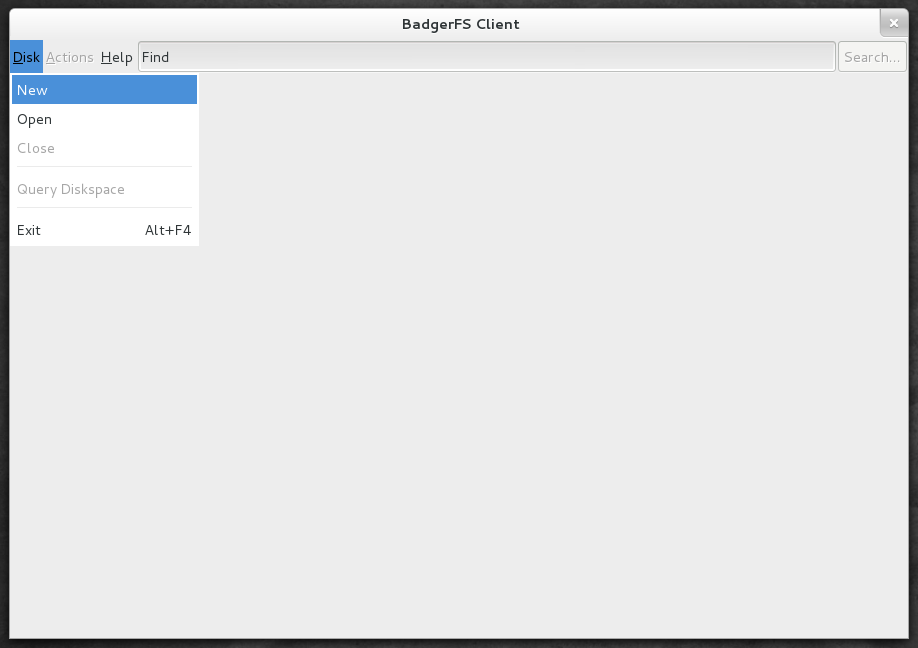
\includegraphics[width=1\textwidth]{figures/01_quickstart.png}
\caption{after startup, create a new disk}
\label{fig:01_quickstart}
\end{figure}

\begin{figure}[h!]
\centering
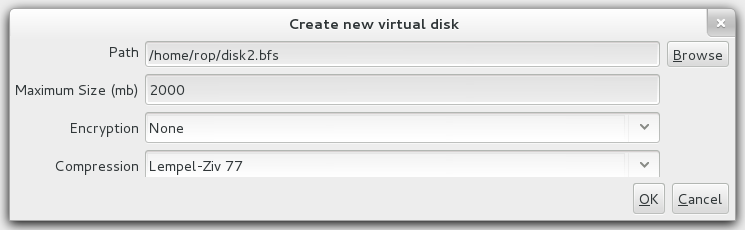
\includegraphics[width=1\textwidth]{figures/02_quickstart.png}
\caption{the disk creation wizard openes, one can choose the file, file size,
encryption and compression algorithms}
\label{fig:02_quickstart}
\end{figure}

\begin{figure}[h!]
\centering
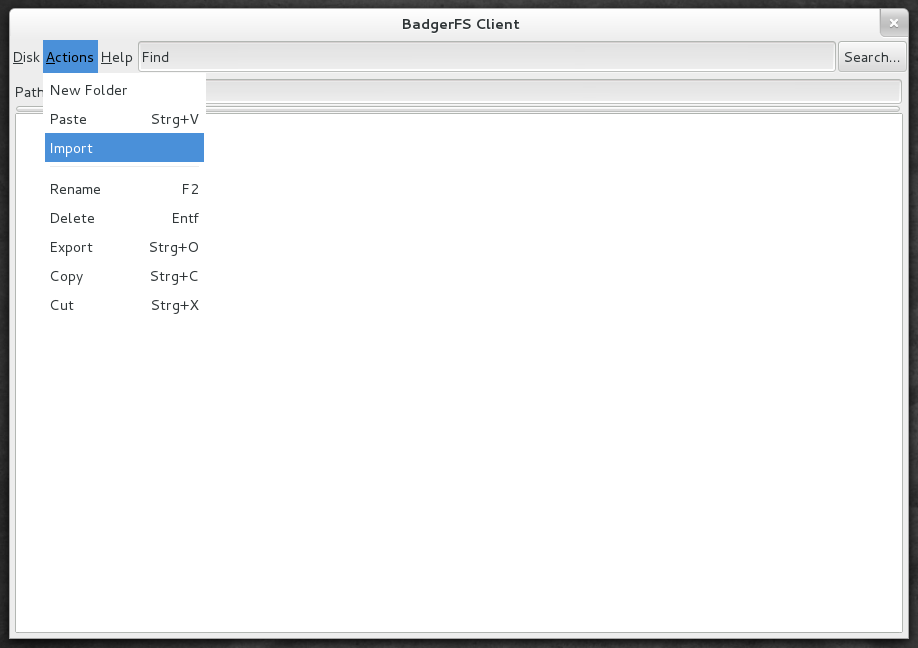
\includegraphics[width=1\textwidth]{figures/03_quickstart.png}
\caption{the new disk gets created on the host filesystem and the user can
start importing files via Actions/Import\ldots}
\label{fig:03_quickstart}
\end{figure}

\begin{figure}[h!]
\centering
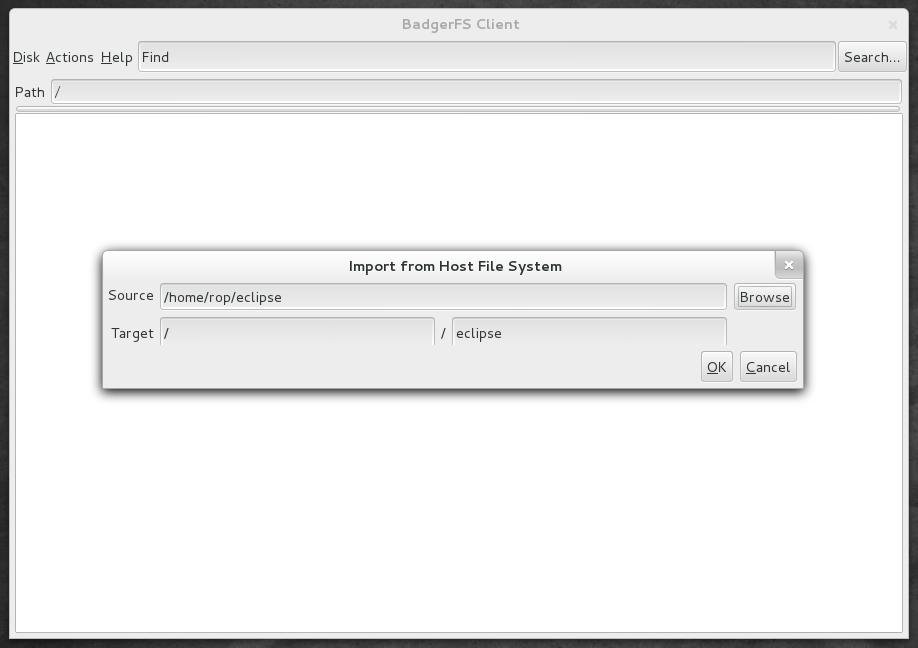
\includegraphics[width=1\textwidth]{figures/04_quickstart.png}
\caption{\ldots which triggers the import dialog, where the user can choose a
file or folder\ldots}
\label{fig:04_quickstart}
\end{figure}

\begin{figure}[h!]
\centering
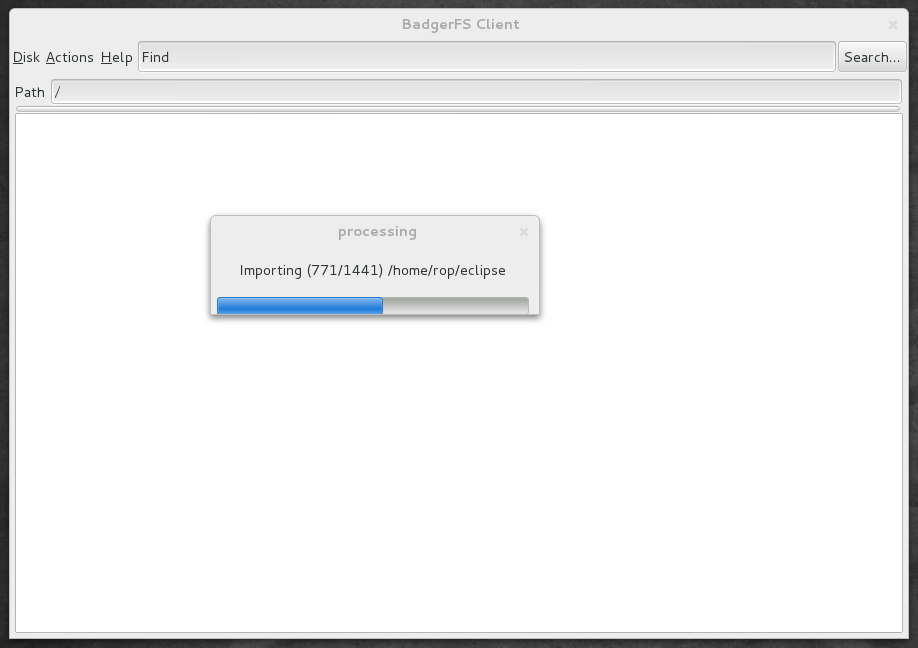
\includegraphics[width=1\textwidth]{figures/05_quickstart.png}
\caption{after clicking ``OK'' the progress window appears\ldots}
\label{fig:05_quickstart}
\end{figure}

\begin{figure}[h!]
\centering
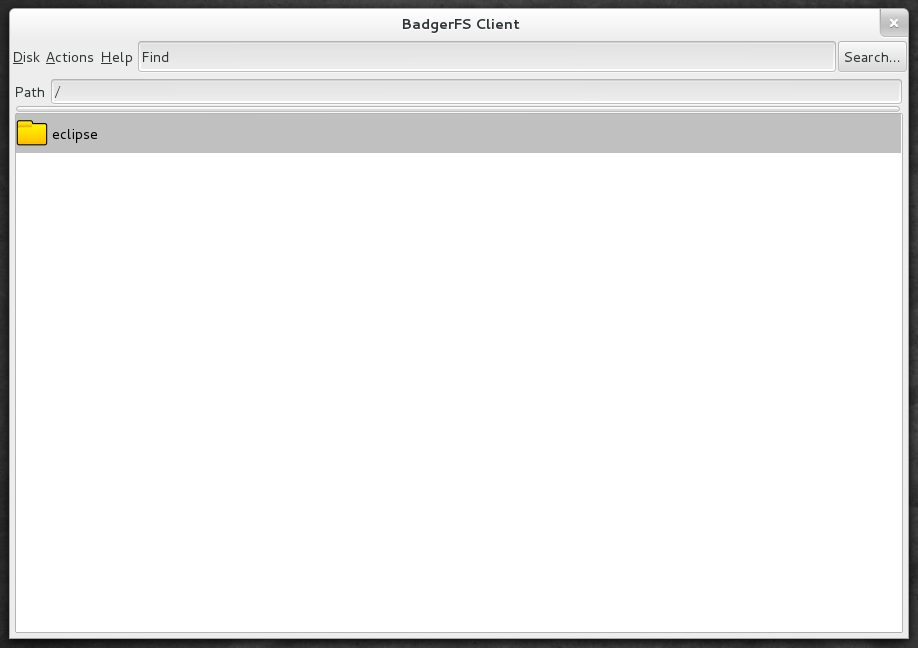
\includegraphics[width=1\textwidth]{figures/06_quickstart.png}
\caption{\ldots and finally the folder is imported after a couple of time.}
\label{fig:06_quickstart}
\end{figure}


\subsection{Disk sychronization}
This section show how to create a new account, log in from two different
machines, import a directory recursively on the first client
and export the directory on the second client. Figures \ref{fig:01_newDisk.png}
through \ref{fig:13_export.png} give a short screenshot view of the steps taken.

Start synchronization server on localhost: Start
\textit{SynchronizationServer} via eclipse. Giving following program arguments
allow some logging output and configuration of the server side files:\newline 
\verb|-l log4j\_server.xml -c /home/rop/Desktop/badger/server/|



\begin{figure}[h!]
\centering
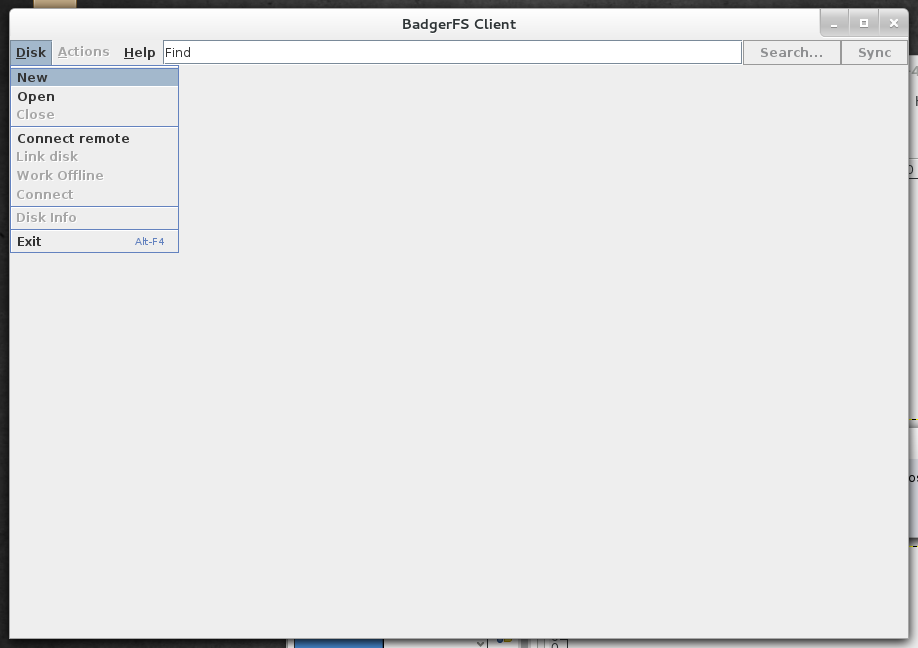
\includegraphics[width=1\textwidth]{figures/serverUseCase/01_newDisk.png}
\caption{Create a new local disk according to figures \ldots}
\label{fig:01_newDisk.png}
\end{figure}

\begin{figure}[h!]
\centering
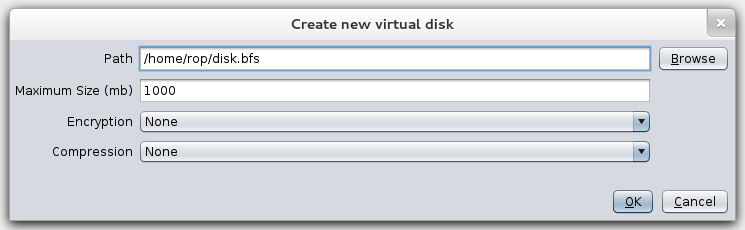
\includegraphics[width=1\textwidth]{figures/serverUseCase/02_newDisk2.png}
\caption{\ldots and set parameters \ldots}
\label{fig:02_newDisk2.png}
\end{figure}

\begin{figure}[h!]
\centering
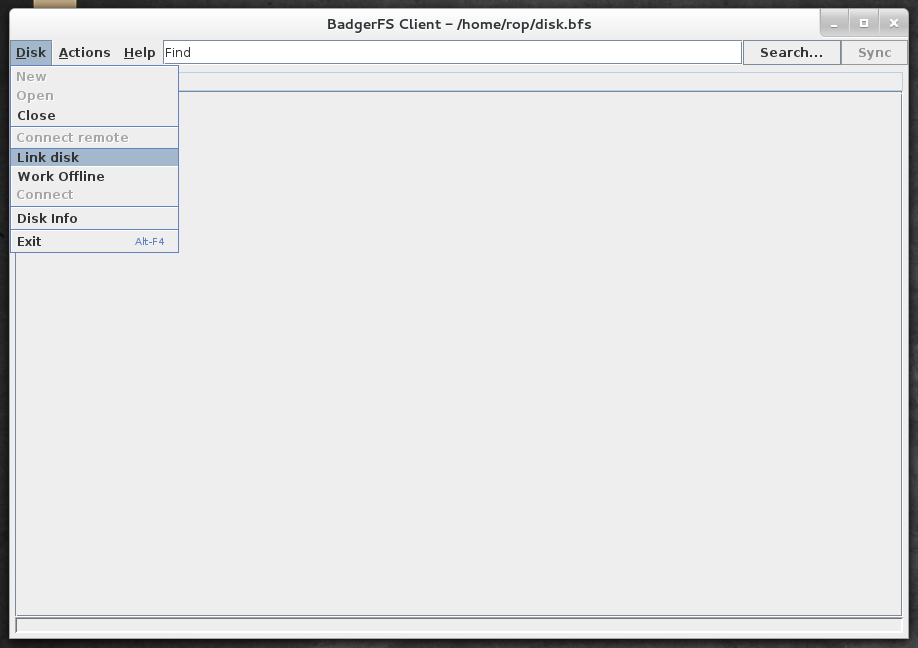
\includegraphics[width=1\textwidth]{figures/serverUseCase/03_linkDisk.png}
\caption{\ldots open ``link disk''\ldots}
\label{fig:03_linkDisk.png}
\end{figure}


\begin{figure}[h!]
\centering
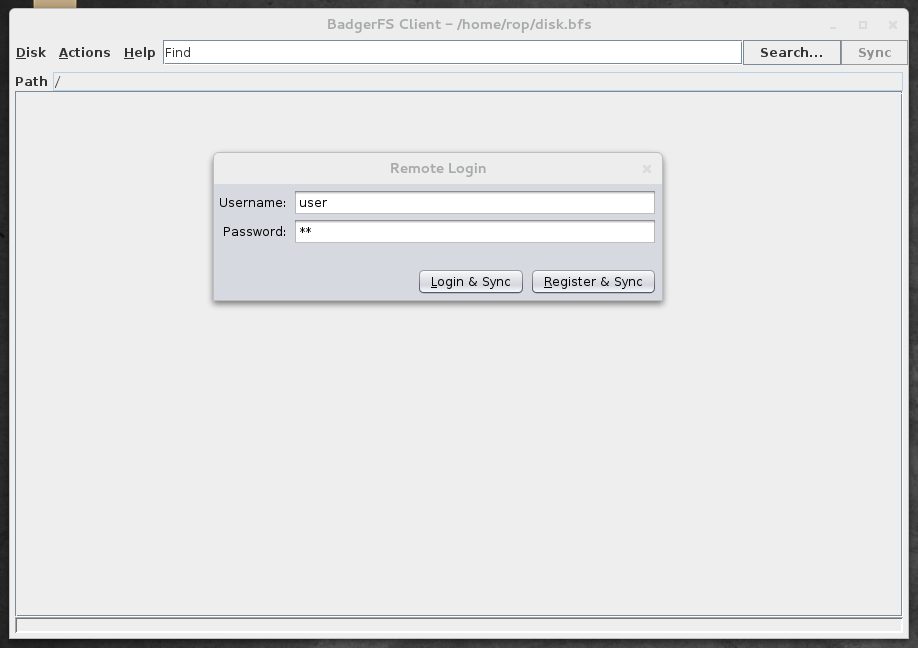
\includegraphics[width=1\textwidth]{figures/serverUseCase/04_loginremote.png}
\caption{\ldots enter new username and password, hit ``Register \& Sync''\ldots}
\label{fig:04_loginremote.png}
\end{figure}

\begin{figure}[h!]
\centering
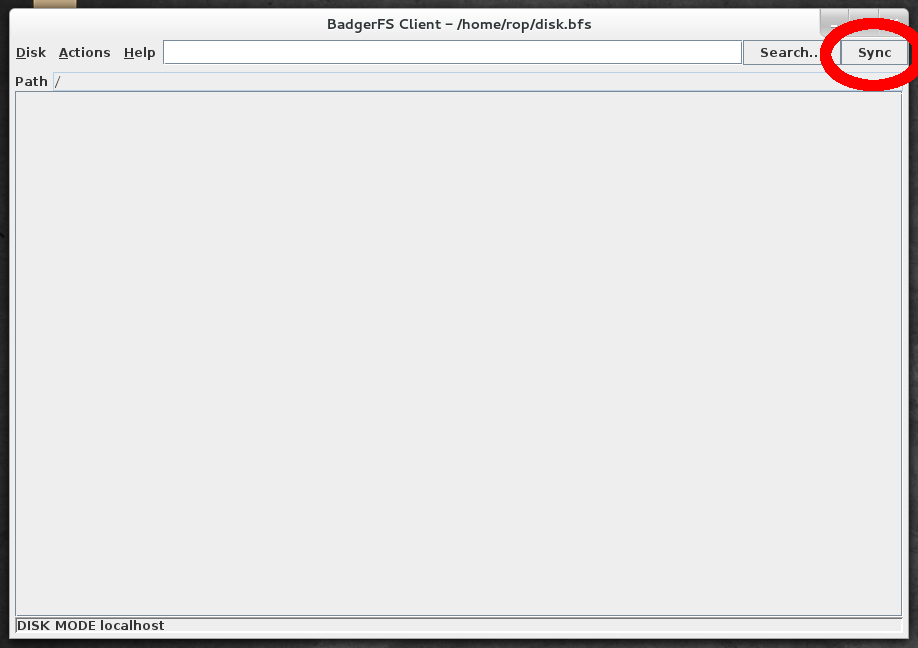
\includegraphics[width=1\textwidth]{figures/serverUseCase/05_linked.png}
\caption{\ldots disk is now linked, ``Sync" button is available\ldots}
\label{fig:05_linked.png}
\end{figure}

\begin{figure}[h!]
\centering
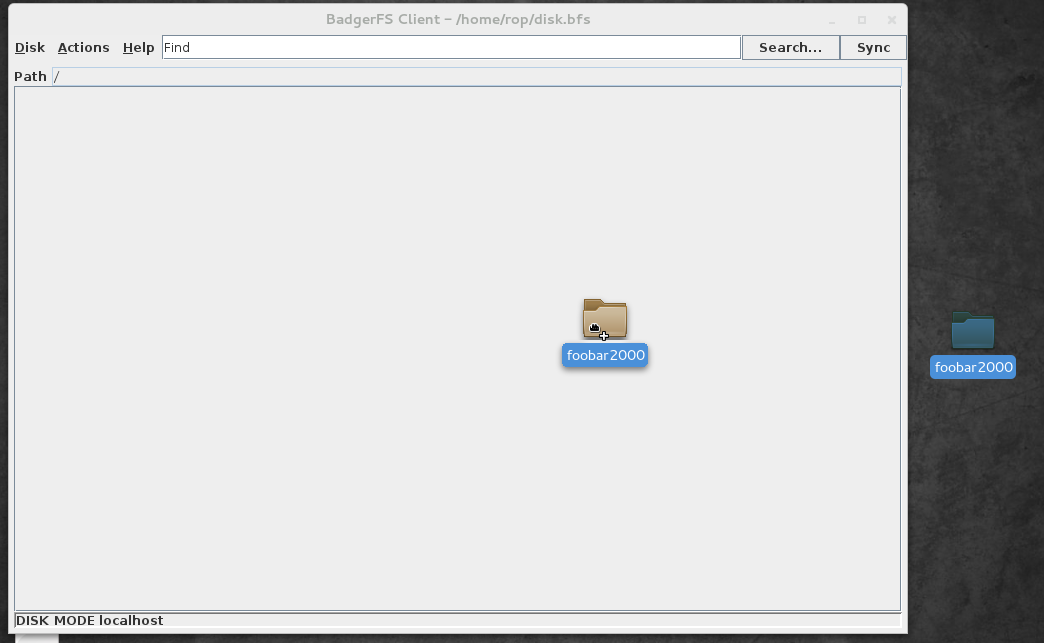
\includegraphics[width=1\textwidth]{figures/serverUseCase/06_dragndrop.png}
\caption{\ldots drag and drop a folder into the grey area\ldots}
\label{fig:06_dragndrop.png}
\end{figure}

\begin{figure}[h!]
\centering
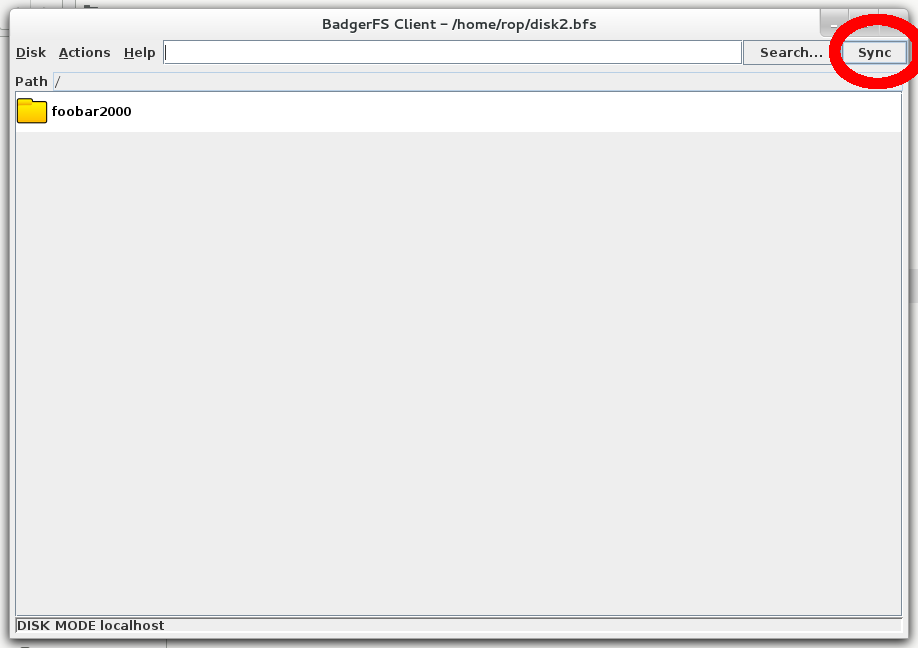
\includegraphics[width=1\textwidth]{figures/serverUseCase/07_sync.png}
\caption{\ldots the folder gets locally imported, and then hit ``Sync" and the
folder gets uploaded \ldots}\label{fig:07_sync.png}
\end{figure}

\begin{figure}[h!]
\centering
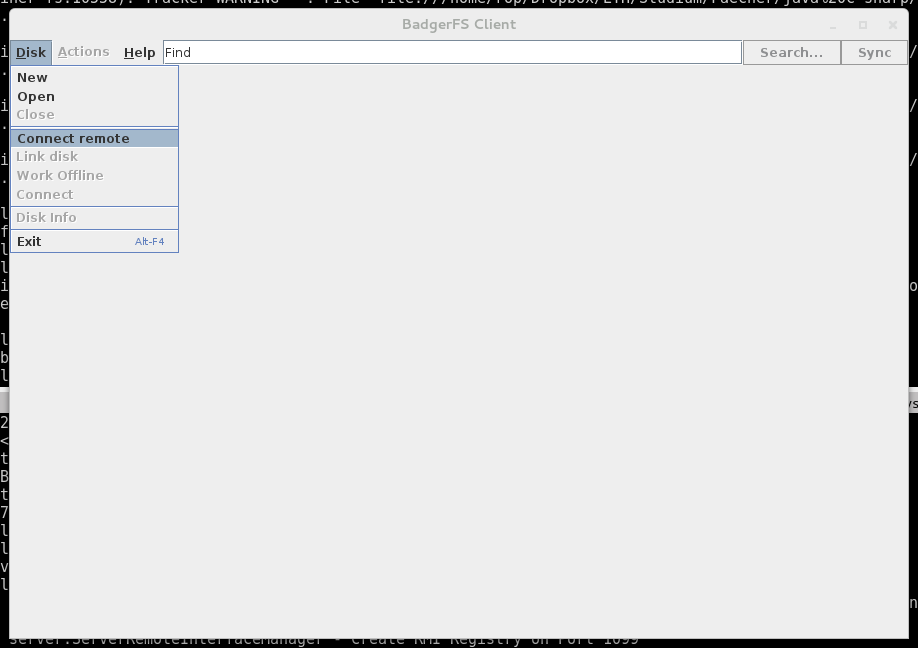
\includegraphics[width=1\textwidth]{figures/serverUseCase/08_new_client_connect_remote.png}
\caption{\ldots in a new client open ``connect remote''
\ldots}\label{fig:08_new_client_connect_remote.png}
\end{figure}


\begin{figure}[h!]
\centering
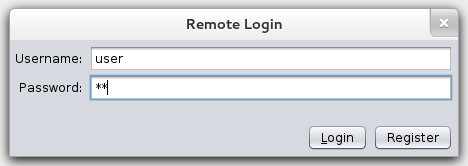
\includegraphics[width=1\textwidth]{figures/serverUseCase/09_login.png}
\caption{\ldots do the login with the old credentials \ldots}
\label{fig:09_login.png}
\end{figure}

\begin{figure}[h!]
\centering
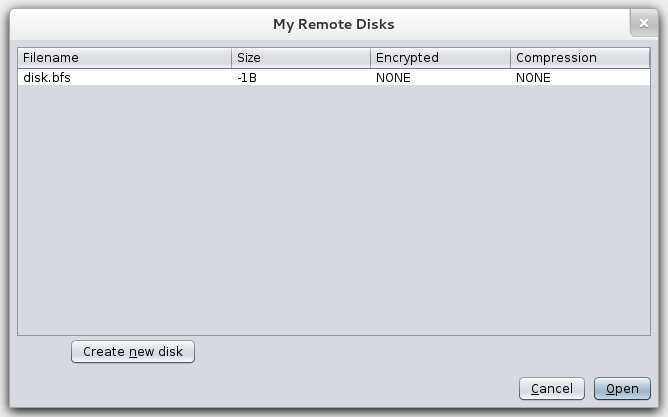
\includegraphics[width=1\textwidth]{figures/serverUseCase/10_choose_disk.png}
\caption{\ldots now you can choose the disk created remotely and open it \ldots}
\end{figure}

\begin{figure}[h!]
\centering
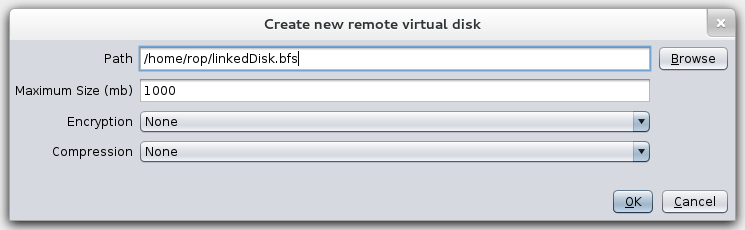
\includegraphics[width=1\textwidth]{figures/serverUseCase/11choose_localdisk.png}
\caption{\ldots here you create a new local disk to synchronize the server file
to \ldots}
\label{fig:11choose_localdisk.png}
\end{figure}

\begin{figure}[h!]
\centering
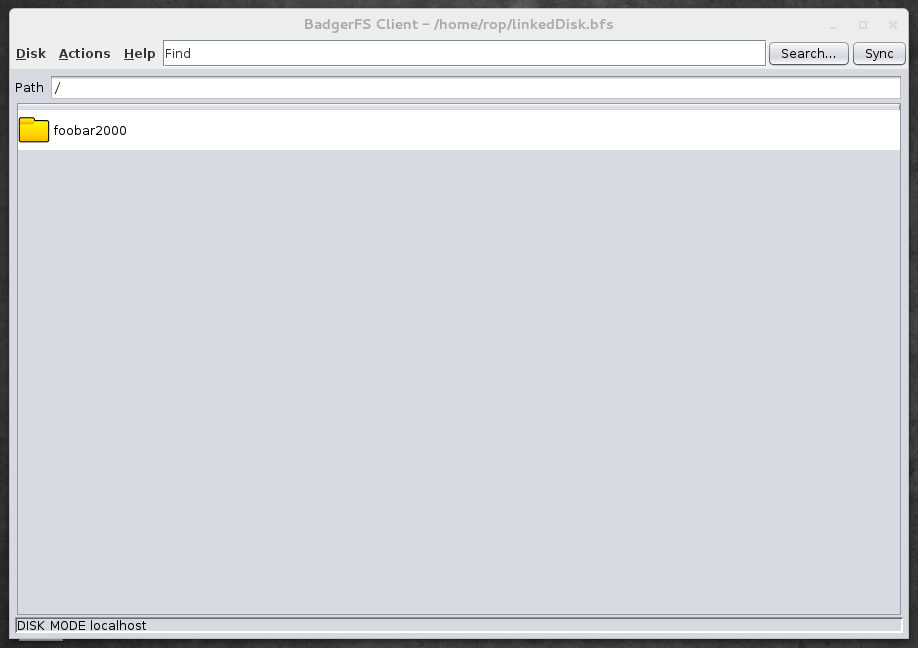
\includegraphics[width=1\textwidth]{figures/serverUseCase/12_sychronized_down.png}
\caption{\ldots upon creation the remote files get synchronized down.}
\label{fig:12_sychronized_down.png}
\end{figure}

\begin{figure}[h!]
\centering
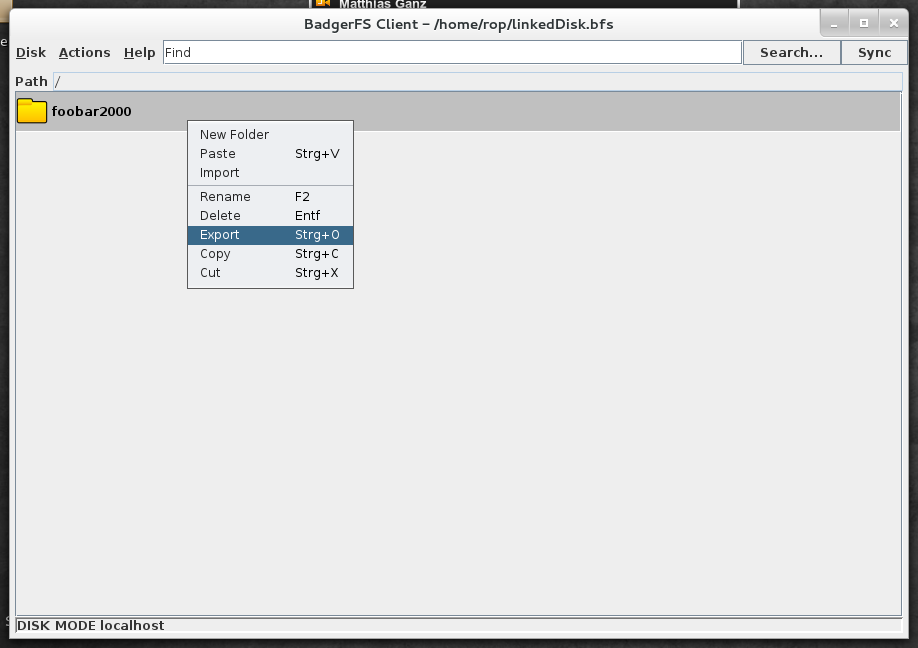
\includegraphics[width=1\textwidth]{figures/serverUseCase/13_export.png}
\caption{ via rightlick - export one can export the freshly created folder.}
\label{fig:13_export.png}
\end{figure}